\chapter{Analytical Model}
\label{ch:analyticalmodel}
%\textit{This chapter presents a calculation of the critical current in a SNS junctions. For this purpose, a quasiclassical transport theory is used and its foundations are explained in the first section. This technique is then employed for a clean SNS junction, and an expression for the Josephson current is found. In the following section, the calculations used for the clean setup are extended for the more sophisticated quantum point contact (QPC) and here as well, the current for the QPC-gated junction is found.}

\section{Foundation of the quasiclassical model}
%This section explains preliminary assumptions made to describe the current in a SNS junction. 
From section \ref{sec:theory-sns} it is known that Andreev reflection of electrons in a SNS junction leads to Andreev bound states within the junction. Each one of these bound states contributes to the total current through the junction. Essentially, a bound state can be expressed as a trajectory from one superconductor through the normal metal to the other superconductor. The superconducting current density is found through geometrical analysis of possible trajectories. The total current density is then found by adding up all these trajectories.
%The superconducting current density is found by summing up these trajectories. This is a way to express the current through geometrical analysis of possible trajectories only. The underlying material does not play a specific role in the calculation, which makes this approach universally applicable.
\begin{figure}[h]
\centering	
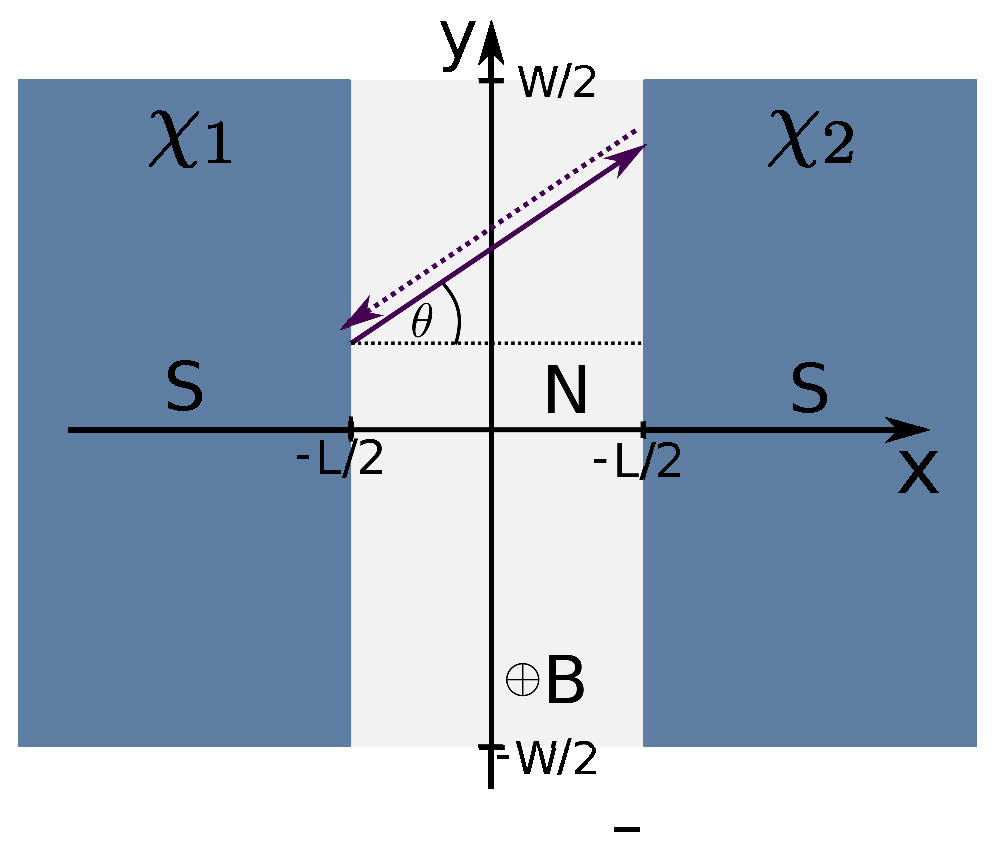
\includegraphics[width=0.6\textwidth]{figure/analyticalmodel/sns_junction}
\caption{Schematic representation of a short and wide SNS junction.}
\label{fig:sns_schematic}
\end{figure}
The two dimensional junction (schematic shown in fig \ref{fig:sns_schematic}) is a short and wide junction with width $W$ and length $L$, where $W \gg L$. The NS-interfaces are parallel to the $y$-axis and are placed at $x = \pm L/2$. Each of the superconducting leads has a phase $\chi_{1}$ and $\chi_{2}$, and the overall phase difference is $\chi = \chi_{1} - \chi_{2}$. The superconducting gap parameter $\Delta$ is only present in the superconducting leads. Close to the interface, $\Delta$ begins to decay on a length scale of the superconducting coherence length $\xi_0$ into the normal region.
%\begin{equation}
%\xi_0 = \hbar v_F / \pi \Delta.
%\end{equation} 
Similar to the procedure in section \ref{sec:theory-sns}, this decay is neglected and a step-like behaviour is assumed for the superconducting gap parameter:
\begin{equation}
\Delta\left( x \right) = |\Delta| e^{\chi_1} \Theta\left(-L/2 -x \right) + |\Delta| e^{\chi_2} \Theta\left(x-L/2 \right).
\label{eq:gap_parameter}
\end{equation}
The thermal length scale of the system assumed to be larger than the sample length:
\begin{equation}
L_T = \hbar v_F / k_B T \gg L.
\end{equation}
The transport through the junction is assumed to be ballistic, resulting in the trajectories being straight and not being altered by scattering in the normal region. However, the presence of the magnetic field in the normal region of the sample will lead to a bending of the trajectories due to the Lorentz force. Depending on the strength of magnetic field $B$ and the Fermi velocity, the radius of this curve is 
\begin{equation}
r_B = \frac{m v_F}{e B}
\end{equation}
In order to justify the assumption of straight trajectories, either the magnetic field has to be weak enough, or the Fermi velocity (wavelength) has to be large (short) enough. Then, the cyclotron radius $r_B$ is larger than the sample size $L$, and straight trajectories are a valid assumption. 

\section{Plane setup: calculation of current}
Summing up the contributions leads to the current through the SNS junctions, the Josephson current $J\left( \chi \right)$, which is a function of the superconducting phase difference $\chi = \chi_2 - \chi_1$. By maximizing the Josephson current with respect to $\chi$, one finds the critical current $I_c$.\\
A trajectory connecting the two superconducting interfaces can be parametrized by the angle $\theta$ between the trajectory and the x-axis. For a trajectory from a point $(-L/2, y_1)$ to another at $(+L/2, y_2)$, the angle for the parametrization is
\begin{equation}
\tan \theta = \frac{y_2 - y_1}{L}.
\label{eq:parametrization}
\end{equation}
Figure \ref{fig:sns_schematic} visualizes this parametrization. 
Several papers outline approaches to this problem (\cite{Zagoskin1997}, \cite{Barzykin1999}) and are based on the same concept. The Josephson current in \cite{Zagoskin1997} has the form
\begin{equation}
J =  \frac{2 e }{\pi L} \sum_{\bm{\kappa}}v^{\bm{\kappa}}_{Fx} \mathcal{J} \left(\chi\right), \label{eq:i-zagoskin}
\end{equation}
where $\bm{\kappa}$ is the tangential momentum with $\bm{\kappa}^2 + \mathbf{k_x}^2 = k_F^2$.
%TODO simply \kappa = k_y?
$v_{Fx}$ is the projection of $v_F$ on the x-axis
\begin{equation}
v_{Fx} =  v_F  \cos \theta
\end{equation}
and $\mathcal{J} \left( \chi \right)$ is the current density. A similar ansatz to eq. (\ref{eq:i-zagoskin}) is described in \cite{Meier2016}:
\begin{equation}
J =  \int_{-W/2}^{+W/2} dy \int_{-p_F}^{+p_F} \frac{dp_y}{2 \pi} \cos \theta \mathcal{J} \left( \chi, \phi \right).
\end{equation}
For a fixed point at the left interface, the current density is integrated over all possible momenta. This integral can be expressed through the endpoints of a trajectory. The integration over $p_y$ can then be replaced by $p_y = p_F \sin \theta \rightarrow d p_y/d\theta = p_F \cos \theta$. The integration over the angle $\theta$ can be substituted by the integration over $y_2$, a point at the right interface. The result for the Josephson current reads
\begin{equation}
J\left(\chi, \phi=0\right) = \frac{2 e v_F}{\pi \lambda_F L^2}  \int \int_{-W/2}^{W/2} d y_1 d y_2 \frac{\mathcal{J}(\chi)}{\left[ 1 + \left(\frac{y_1 - y_2}{L}\right)^2\right]^2}.
\label{eq:josephson_current_zero_b}
\end{equation}
By maximizing the Josephson current with respect to $\chi$, the critical current can be found as:
\begin{equation}
I_c(\phi) = \text{max}_{\chi}\left\{ J(\chi, \phi) \right\}\label{eq:josephson-relation}.
\end{equation} 
%TODO insert result of integration with B=0
The current density $\mathcal{J}$ depends on the ratio of $W$ and $L$. For $W \gg L$, the junction is a short junction, while for $W \ll L$, it is a long junction. 
In the short junction limit, the current density is calculated in \cite{Beenakker1991}
\begin{equation}
\mathcal{J}^s (\chi) = \frac{\mathcal{T}_n \sin \chi}{\sqrt{1 - \mathcal{T}_n \sin^2 \frac{\chi}{2}}}
\end{equation}
which can be derived in the framework of the scattering matrix formalism. $\mathcal{T}_n$ is the transmission coefficient for a given conducting channel. For low transmission, $\mathcal{T} \ll 1$, only the first addend contributes, which leads to the conventional Josephson relation $J \simeq \mathcal{T} \sin \chi$.\\
For the long junction, from \cite{Barzykin1999} the following expression can be found:
\begin{equation}
\mathcal{J}^l(\chi) = \sum_{k = 1}^{\infty} \frac{(-1)^{k+1}}{k} \sin( k \chi).
\end{equation}
The coefficient $\mathcal{T}$ has been included phenomenologically in this formula and includes the normal scattering in the sample.
\begin{figure}
\centering
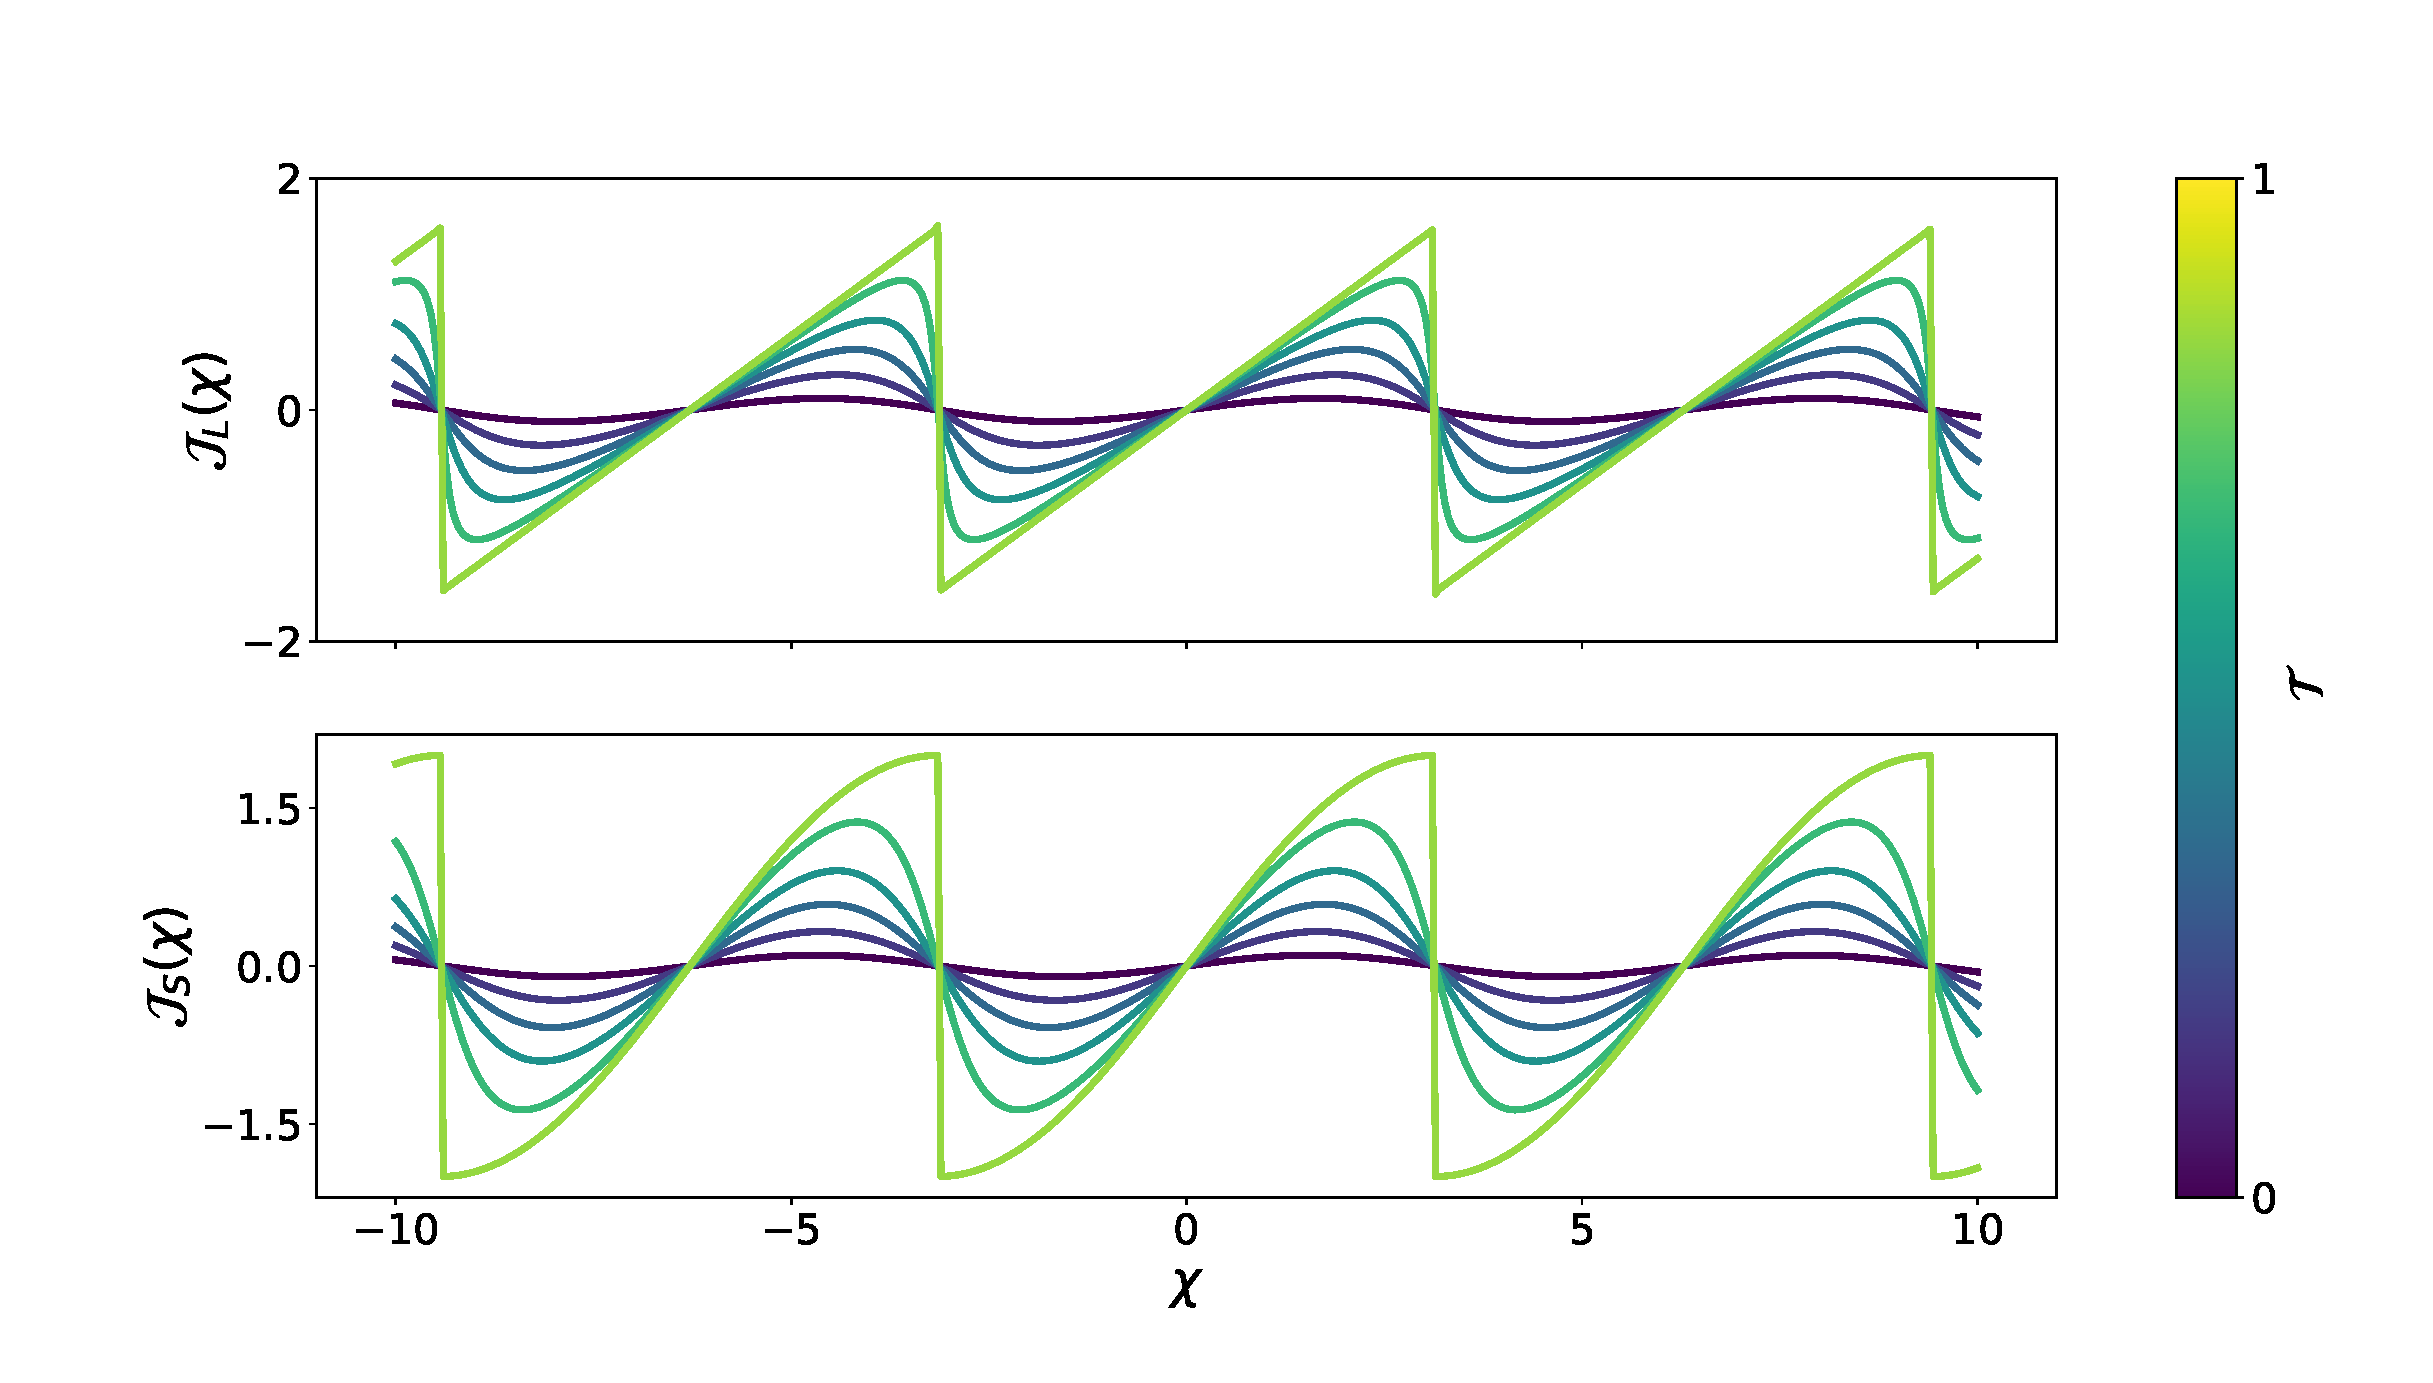
\includegraphics[width=\textwidth]{figure/analyticalmodel/current_density_all}
\caption{Short and long junction current density}
\label{fig:current_density}
\end{figure}
Figure \ref{fig:current_density} shows a plot of both short and long junction limit current densities. For $\mathcal{T} \ll 1$, $\mathcal{J}^s$ takes a sinusoidal form, which also true for the long junction limit. For each of those, the classical Josephson relation can be found in the limit of low transmissions. The current densities differ for a large transmission coefficient $\mathcal{T} \simeq 1$: A sawtooth-like shape is observed in the long junction limit, and in the short junction limit, a sinusoidal shape appears.\\

%%%%%
\subsection*{Including magnetic field}
Up to this point, the current has been derived for zero magnetic field. If a finite magnetic field is considered, the phase $\chi$ is modified because of two effects: First, the magnetic phase that will be acquired along a trajectory connecting two points $y_1$ and $y_2$  leads to an additional term in the phase. Also, the superconducting phases at each interface become functions of $y_{1/2}$ (see \cite{Meier2016}):
%Then again, \textit{the condition of zero screening current in the bulk superconducting region and the limit of} $\lambda_L \rightarrow 0$ \textit{require the superconducting phase at the interfaces to become functions of y.
\begin{eqnarray}
\chi_{1/2} &=& \mp \frac{1}{2}\left( \chi - \frac{2 \pi B L }{\phi_0} y_{1/2}\right) \\
\tilde{\chi}(y_1, y_2) &=& \chi_2 - \chi_1 \\
 &=& \chi - \frac{\pi B L}{\phi_0}(y_1 + y_2)
 \label{eq:chi}
\end{eqnarray}
Assuming that the London penetration depth is small to zero in the superconducting regions, the following gauge for the vector potential can be used:
\begin{equation}
\mathbf{A}=A_y \mathbf{e}_y, \quad
A_y=\left\{ 
		\begin{array}{ll}
				-B x, & -L/2 \leq x \leq L/2, \\[0.2cm] 
				-\frac{1}{2} B L |x| , & \quad |x|>L/2
		\end{array} 
	\right.
\label{eq:Ay}
\end{equation}
This gauge will give no additional contribution to the phase on straight trajectories
\begin{eqnarray}
\delta \chi &=& \frac{2 \pi}{\Phi_0} \int d \mathbf{l} \cdot \mathbf{A} \\
&=& \frac{2 \pi}{\Phi_0} \int_{-L/2}^{L/2} \frac{dx}{\cos \theta} A_y (x) \sin \theta \\
&=& - \frac{2 \pi B}{\Phi_0} \frac{y_2 - y_1}{L} \int_{-L/2}^{L/2} x dx \\
&=& 0, 
\end{eqnarray}
where eq.~(\ref{eq:parametrization}) has been used. The total phase for this setup is therefore eq.~(\ref{eq:chi}). This results in the current phase relation in the expression for the Josephson current from eq. (\ref{eq:josephson_current_zero_b}) to be replaced by the effective phase $\chi \rightarrow \tilde{\chi}(y_1, y_2)$:
\begin{equation}
J\left(\chi, \phi \right) = \frac{2 e v_F}{\pi \lambda_F L^2}  \int \int_{-W/2}^{W/2} d y_1 d y_2 \frac{\mathcal{J}(\tilde{\chi}(y_1, y_2))}{\left[ 1 + \left(\frac{y_1 - y_2}{L}\right)^2\right]^2}
\label{eq:josephson_current}
\end{equation}
By maximizing the Josephson current with respect to $\chi$, the critical current can be found as:
\begin{equation}
I_c(\phi) = \text{max}_{\chi}\left\{ J(\chi, \phi) \right\}
\end{equation}
%\textbf{TODO: Dependence on W/L ratio? Plot of current?}

\section{Calculation of QPC current}
\begin{figure}
\centering
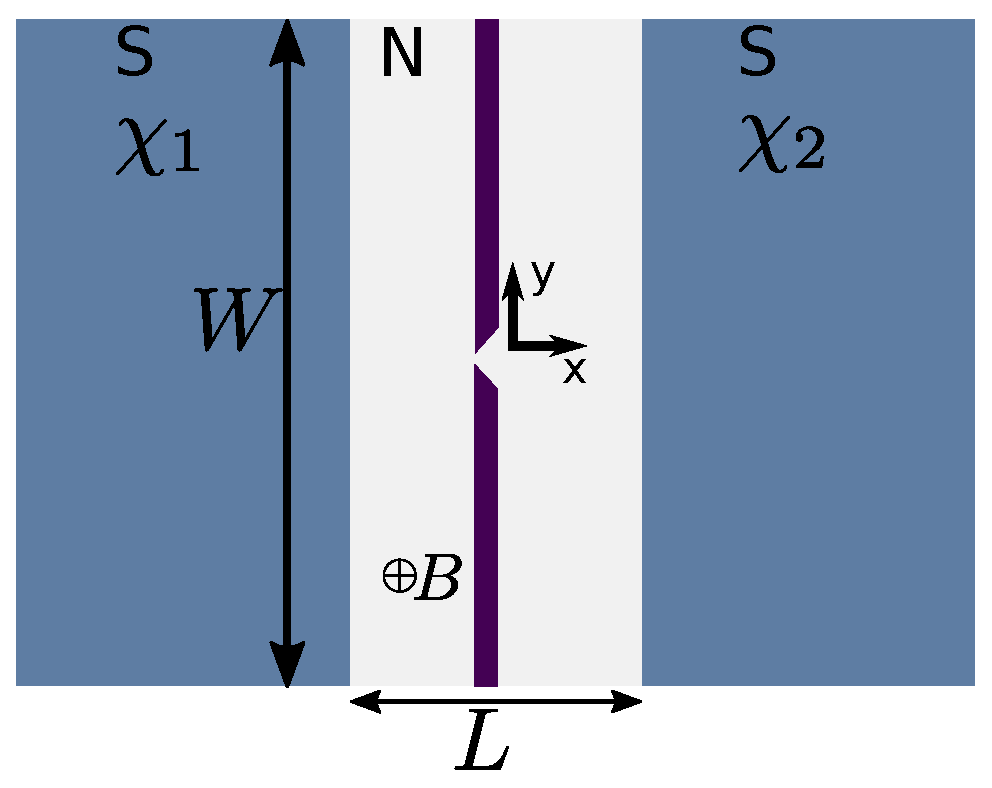
\includegraphics[width=0.6\textwidth]{figure/analyticalmodel/qpc_sns_junction}
\caption{QPC setup.}
\label{fig:qpc_sns_schematic}
\end{figure}
%\textbf{TODO: what happens when a constriction is on top of normal layer, fermi levels etc}
The quasi classical formalism can even be employed to modified SNS junctions. One can build gates on top of the normal region of the junction in a way that the current cannot pass through the gated regions (see chapter \ref{ch:experiment}). In the quasi classical picture, this means that the possibilities for trajectories connecting two points at the superconducting interfaces are limited through the geometry of the constriction.\\
Figure \ref{fig:qpc_sns_schematic} shows a sketch of the quantum point contact set-up which will be analysed with the quasi classical formalism. The normal region of the SNS junction is covered by a gate with a small split in the middle. The split is located at $(x, y) = (0, 0)$ so that the sample is symmetric around the origin. The width of the split is in the order of $\lambda_F$  and can thereby be viewed as an isotropic scattering point with transmission coefficient $\mathcal{T}_0$. Trajectories connecting the two superconducting interfaces have to pass through the QPC. For simplicity, the geometrical width of the barrier is neglected, only straight trajectories are considered, and scattering at side edges is neglected. This modified set-up leads to a different parametrization of the trajectories and therefore to a different magnetic phase than in eq. (\ref{eq:chi}).\\
With the QPC set-up, all possible trajectories are parametrized by two angles $\theta_1$ and $\theta_2$. $\theta_1$ describes the trajectory before passing through the QPC in the region $ -L/2 < x < 0$, and  $\theta_2$ after passing through the QPC. The parametrization of the trajectories reads
\begin{equation}
\tan \theta_1 = - \frac{2 y_1}{L}, \quad \tan \theta_2 = \frac{2 y_2}{L}
\label{eq:QPCparametrization}
\end{equation}
With the gauge from eq. (\ref{eq:Ay}), the magnetic phase acquired within the sample reads
\begin{eqnarray}
\frac{2\pi}{\Phi_0} \int d\mathbf{l} \cdot \mathbf{A}  &=&
-\frac{\pi B}{\Phi_0}\left(\frac{L}{2}\right)^2
\left(-\tan\theta_1 + \tan\theta_2\right) =
-\frac{\pi \phi (y_1+y_2)}{2 W}.
\label{eq:phaseQPC}
\end{eqnarray}
Adding this contribution to the term in eq.~(\ref{eq:chi}), the effective phase for the QPC setup is found to be
\begin{equation}
\tilde{\chi}(y_1,y_2)=\chi-\frac{3 \pi \phi }{2W}(y_1+y_2).
\label{eq:chiQPC}
\end{equation}
%The contribution in eq. (\ref{eq:chiQPC}) is half of the effective phase without any constriction, as written in eq. (\ref{eq:chi}). This is reasonable and can be illustrated by looking at the area contributing to the phase. Only half of the normal region is covered by all possible trajectories in the QPC case, whereas in the case without any constriction, the whole normal region contributes.\\
%\textbf{TODO: stimmt das da oben? warum?}\\
One consequence of the additional gate on top of the normal region is the change in the effective phase, resulting in a modified current phase relation $\mathcal{J}(\tilde{\chi}(y_1, y_2))$. Another consequence is a modified expression for the critical current. In the set-up without gates, straight trajectories with a fixed angle $\theta$ were considered and summed up to a total contribution. The difference in the QPC set-up is the split in the gate, which is modelled as an isotropic scattering point. The trajectories being summed up in this set-up can be thought to consist of two parts. The first part connects $y_1$ with the split at $(x, y) = (0, 0)$ and is determined by the direction of the trajectory. This explains the Fermi velocity in this part(?). The second part of the current trajectory starts from the origin and connects it with a point at the right interface $y_2$. Summing up, the  critical current in the QPC set-up is
\begin{equation}
I_c^{\text{QPC}}(\phi) \propto \text{max}_{\chi} \int d \theta_1 v_F \cos^2 \theta_1 \int d \theta_f \cos \theta_f \mathcal{J}\left( \tilde{\chi} (\theta_1, \theta_2) \right)
\end{equation}
%The normalized critical current reads
%\begin{eqnarray}
%\frac{I_c(\phi)}{I_c(0)} &=& \frac{ \text{max}_{\chi} \int d \theta_i \cos^2 \theta_i\int d \theta_f \cos \theta_f \mathcal{J}(\tilde{\chi}(\theta_i, \theta_f)) }{ \text{max}_{\chi} \int d \theta_i \cos^2 \theta_i\int d \theta_f \cos \theta_f \mathcal{J}(\chi) }
%\end{eqnarray}
The QPC is modelled as an isotropic scatterer with transmission probability $\mathcal{T}$. If the transmission is small, $\mathcal{T} << 1$, eq.~(\ref{eq:josephson-relation}) can be used for $\mathcal{J}$.
%TODO \textbf{TODO: add why from $\sin \tilde{\chi}$ only cosine survives!}
The angles $\theta_{1, 2}$ can be rewritten in terms of $y_{1, 2}$ by using the parametrization from eq.~(\ref{eq:QPCparametrization}), allowing the normalized critical current to be expressed as
\begin{eqnarray}
\frac{I_c(\phi)}{I_c(0)} &=& \frac{\mathcal{I}_2(\phi)\mathcal{I}_{3/2}(\phi)}{\mathcal{I}_2(0)\mathcal{I}_{3/2}(0)},
\end{eqnarray}
where the integrals $\mathcal{I}$ are defined as
\begin{equation}
\mathcal{I}_k(\phi) = \frac{2}{L}\int_{-W/2}^{+W/2}dy \frac{\cos\left(\frac{3\pi\phi y}{2W}\right)}{\left[1 + \left(\frac{2y}{L}\right)^2 \right]^k}
\label{integral-qpc}
\end{equation}
The current can be evaluated in the limit of small flux $\phi \rightarrow 0$, and in limit of high fields $\phi \rightarrow \infty$. 
At $\phi=0$ the cosine term becomes one leading to the simple expression
\begin{eqnarray}
\mathcal{I}_2(0)\mathcal{I}_{3/2}(0) &=&
\frac{2 W}{\sqrt{L^2+W^2}}\arctan\frac{W}{L} + \frac{2 L W^2}{(L^2+W^2)^{3/2}} \\
&\equiv& \frac{2x}{\sqrt{1 + x^2}} \arctan x + \frac{2 x^2}{\left( 1 + x^2 \right)^{3/2}}, \quad x = W/L
\label{Ic-0}
\end{eqnarray}
The parabolic asymptotics of the critical current at small $\phi$ is found by expanding the cosine factors in the numerator:
\begin{eqnarray}
\frac{I_c(\phi)}{I_{c0}}&\simeq& 1 - \frac{9\pi ^2 \phi^2 }{32} f_0(W/L) \\
f_0(x) &=& \frac{\sqrt{x^2+1} \log \left(\sqrt{x^2+1}+x\right)}{x^3} - \frac{2}{x (x+(x^2+1) \arctan x)} 
\end{eqnarray}
In the opposite limit of high fields, $\phi\to \infty$, the integration in eq.~(\ref{integral-qpc}) is extended over $y_1$ and $y_2$ to $\pm \infty$ and obtain
\begin{eqnarray}
\frac{I_c(\phi)}{I_{c0}} &=& \frac{\pi^2 \left(1+x^2\right)^{3/2}}{4x\left(x + \left(1+x^2\right)\arctan x\right)}\left(1 + \frac{3 \pi \phi }{4 x} \right) \sqrt{\frac{3 \phi}{2x}}\exp\left(-\frac{3\phi\pi}{2x}\right)
\label{large-phi}
\end{eqnarray}
%\textbf{TODO: write this one in pretty}
\newpage
\section{QPC edge current}
Additionally to the QPC, two edge channels at $(x, y) = (0, \pm w/2)$ are introduced. The QPC is modelled with the transmission coefficient $\mathcal{T}_q$, and the edge channel with the coefficient $\mathcal{T}_e$. The lattice orientation of the graphene structure may may be either predominantly arm-chair or zigzag. Depending on this orientation, the edge currents may or may not contribute significantly  to the total current. The Fraunhofer pattern changes accordingly.

%TODO cite!
\begin{figure}
\centering
\includegraphics[width=0.5\textwidth]{figure/analyticalmodel/qpc_edges_angles}\label{fig:qpc-edge-parametrization}
\caption{A figure caption.}
\end{figure}
The parametrization of an edge trajectory, illustrated in figure \ref{fig:qpc-edge-parametrization}, reads
\begin{eqnarray}
\tan \theta_1 = ~\frac{ W - y_1}{L/2}, \quad \tan \theta_2 = -\frac{W - y_2}{L/2} \label{eq:angles-edge}.
\end{eqnarray}
Similar to the QPC contribution, the magnetic phase gain along the trajectory is calculated. For the upper edge, the result is
\begin{eqnarray}
\frac{2 \pi}{\phi_0} \int d \mathbf{l} \cdot \mathbf{A} &=& \frac{2 \pi}{\phi_0} \left( \int A_y(x) |d\mathbf{l}| |\mathbf{e_y}| \sin \theta_1 + \int A_y(x) |d\mathbf{l}| |\mathbf{e_y}| \sin \theta_2  \right)\\
%&=& \frac{2 \pi B}{\phi_0} \left( \int_{-L/2}^{0} \frac{x dx}{\cos \theta_1} \sin \theta_1  + \int_{0}^{L/2} \frac{x dx}{\cos \theta_2} \sin \theta_2 \right) \\
&=&  - \frac{2 \pi B}{\phi_0} \left( \int_{-L/2}^{0} x dx \tan \theta_1 + \int_{0}^{L/2} x dx \tan \theta_2 \right) \\
&=&  - \frac{\pi B}{\phi_0} \frac{L}{2} \left( - \tan \theta_1 + \tan \theta_2 \right) \\
&=& - \frac{\pi B}{\phi_0} \frac{L}{2} \left( -2W + (y_1 + y_2) \right)\\
&=& \pi \Phi -\frac{\pi \Phi }{2 W} (y_1 + y_2),
\end{eqnarray}
where
\begin{equation}
\Phi = \frac{\phi}{\phi_0}, \quad \phi = B W L
\end{equation}
has been used. Together with the contribution from the set-up without any constriction from eq.~(\ref{eq:chi}), the total phase for the edge transmission is added up to
\begin{equation}
\tilde{\chi}(y_1, y_2) = \chi - \frac{3 \pi \Phi}{2\phi_0} (y_1 + y_2) + \pi \Phi \label{eq:chi-edge}.
\end{equation}
This is the effective phase $\tilde{\chi}(y_1, y_2)$ for the upper edge. Analogously, the phase for the lower edge can be constructed with a simple sign change in the parametrization in eq. (\ref{eq:angles-edge}), leading to
\begin{equation}
\tilde{\chi}(y_1, y_2) = \chi + \frac{3 \pi \Phi}{2\phi_0} (y_1 + y_2) - \pi \Phi \label{eq:chi-edge}
\end{equation}
The Josephson relation for the edge contribution has the modified phase from eq. (\ref{eq:chi-edge}). 
The result for the QPC in the limit in high fields, eq. (\ref{large-phi}), has a transmission coefficient $\mathcal{T} = 1$. For easier comparison with the edge channel contribution, this is rewritten into the following form
\begin{equation}
I_c^{\text{QPC}} = \mathcal{T}_q F(W/L)
\end{equation}
The integrals for the upper edge current at high fields look very similar to the QPC result.
\begin{eqnarray}
I_c^e &=& \mathcal{T}_e \sin \left( \chi_0 - \pi \Phi \right) \int_0^\infty d \tilde{y}_1 \int_0^\infty d \tilde{y}_2 \frac{\cos \left( \frac{3 \pi \Phi \tilde{y}_1}{2 W} \right) }{\left( 1 + \left( \frac{2 \tilde{y}_1}{L}\right)^2 \right)^2} \frac{\cos \left( \frac{3 \pi \Phi \tilde{y}_2}{2 W} \right)}{\left( 1 + \left( \frac{2 \tilde{y}_1}{L}\right)^2 \right)^{3/2}} \\
&=& \mathcal{T}_e \sin \left( \chi_0 - \pi \Phi \right) \frac{F(W/L)}{4}, 
\end{eqnarray}
where
\begin{equation}
\tilde{y}_{1/2} = W/2 - y_{1/2} 
\end{equation}
The total critical current though the junction is proportional to the sum of the individual contributions
\begin{eqnarray}
\frac{I_c\left( \phi \right)}{I_{c0}} &=& \text{max}_\chi \left\{ \mathcal{T}_q \sin \chi + \frac{\mathcal{T}_e}{4} \sin \left( \chi - \pi \phi \right) + \frac{\mathcal{T}_e}{4} \sin \left( \chi + \pi \phi \right) \right\} / \left( \mathcal{T}_q + \mathcal{T}_e/2 \right)\\
&=& \frac{\mathcal{T}_q / \mathcal{T}_e + \cos \left( \pi \phi \right)/ 2 }{\mathcal{T}_q / \mathcal{T}_e + 1/2}\label{eq:ratio-transmissions}
\end{eqnarray}
\begin{figure}
\centering
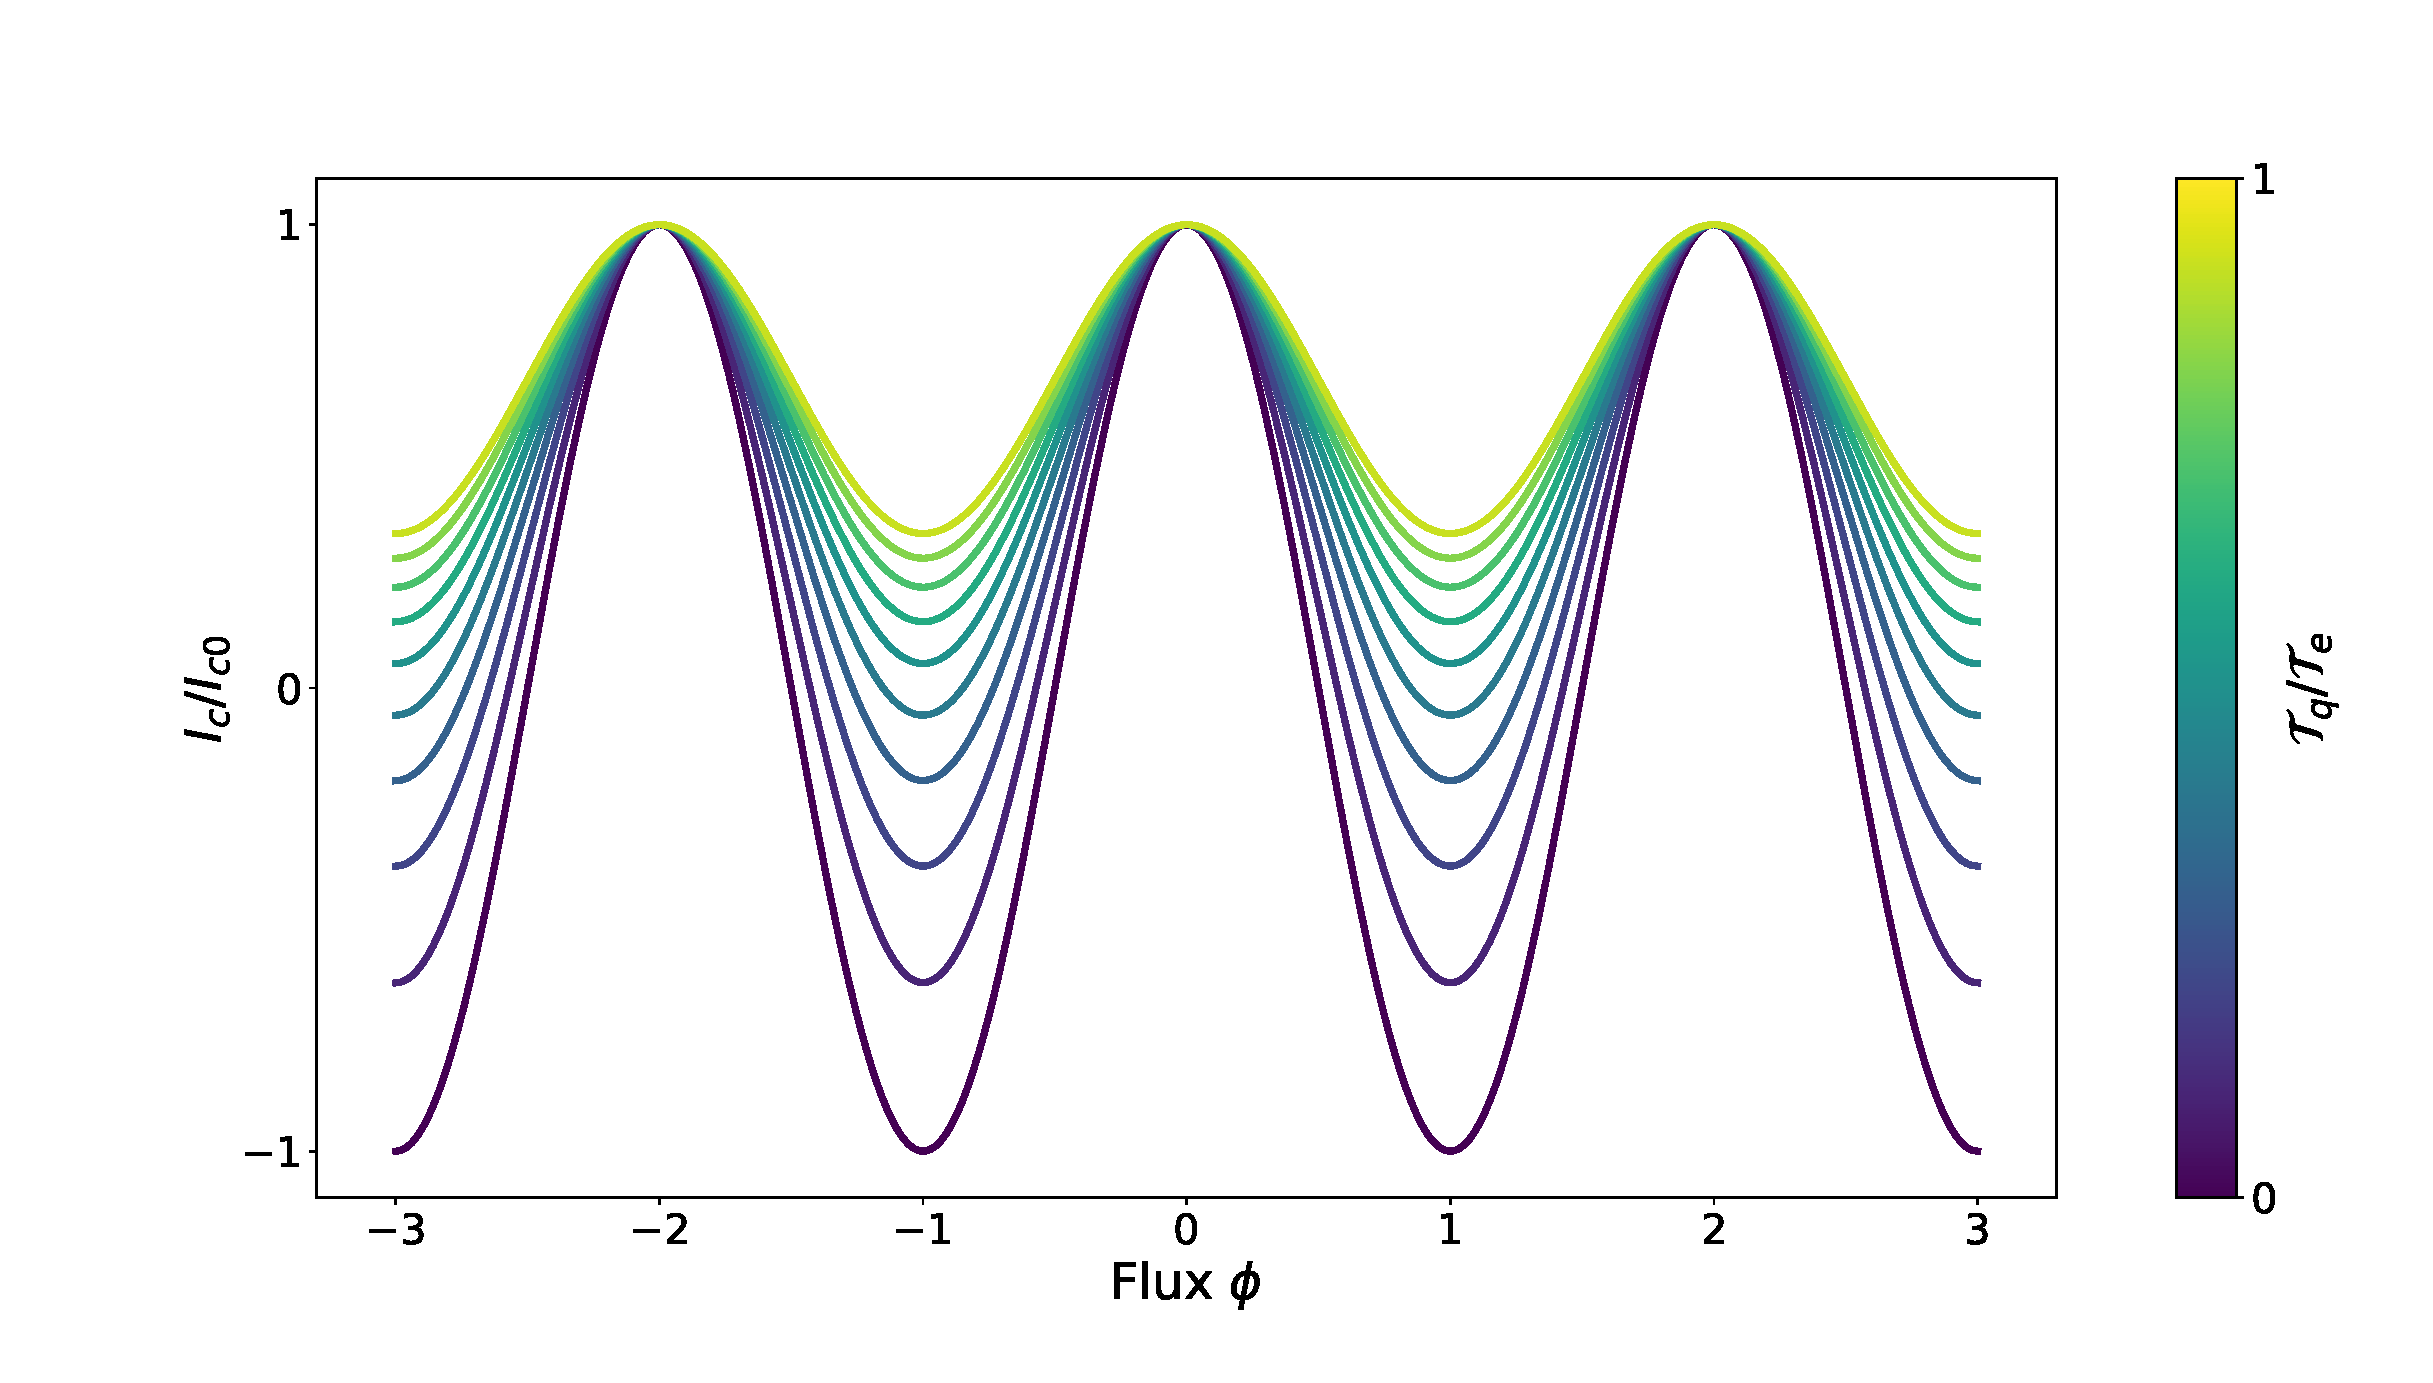
\includegraphics[width=0.8\textwidth]{figure/analyticalmodel/ratio-transmissions} \label{fig:ratio-transmissions}
\end{figure}
The result of eq. (\ref{eq:ratio-transmissions}) is plotted in figure \ref{fig:ratio-transmissions}. 
%For $\mathcal{T}_q/\mathcal{T}_e \ll 1$
\begin{figure}
\centering
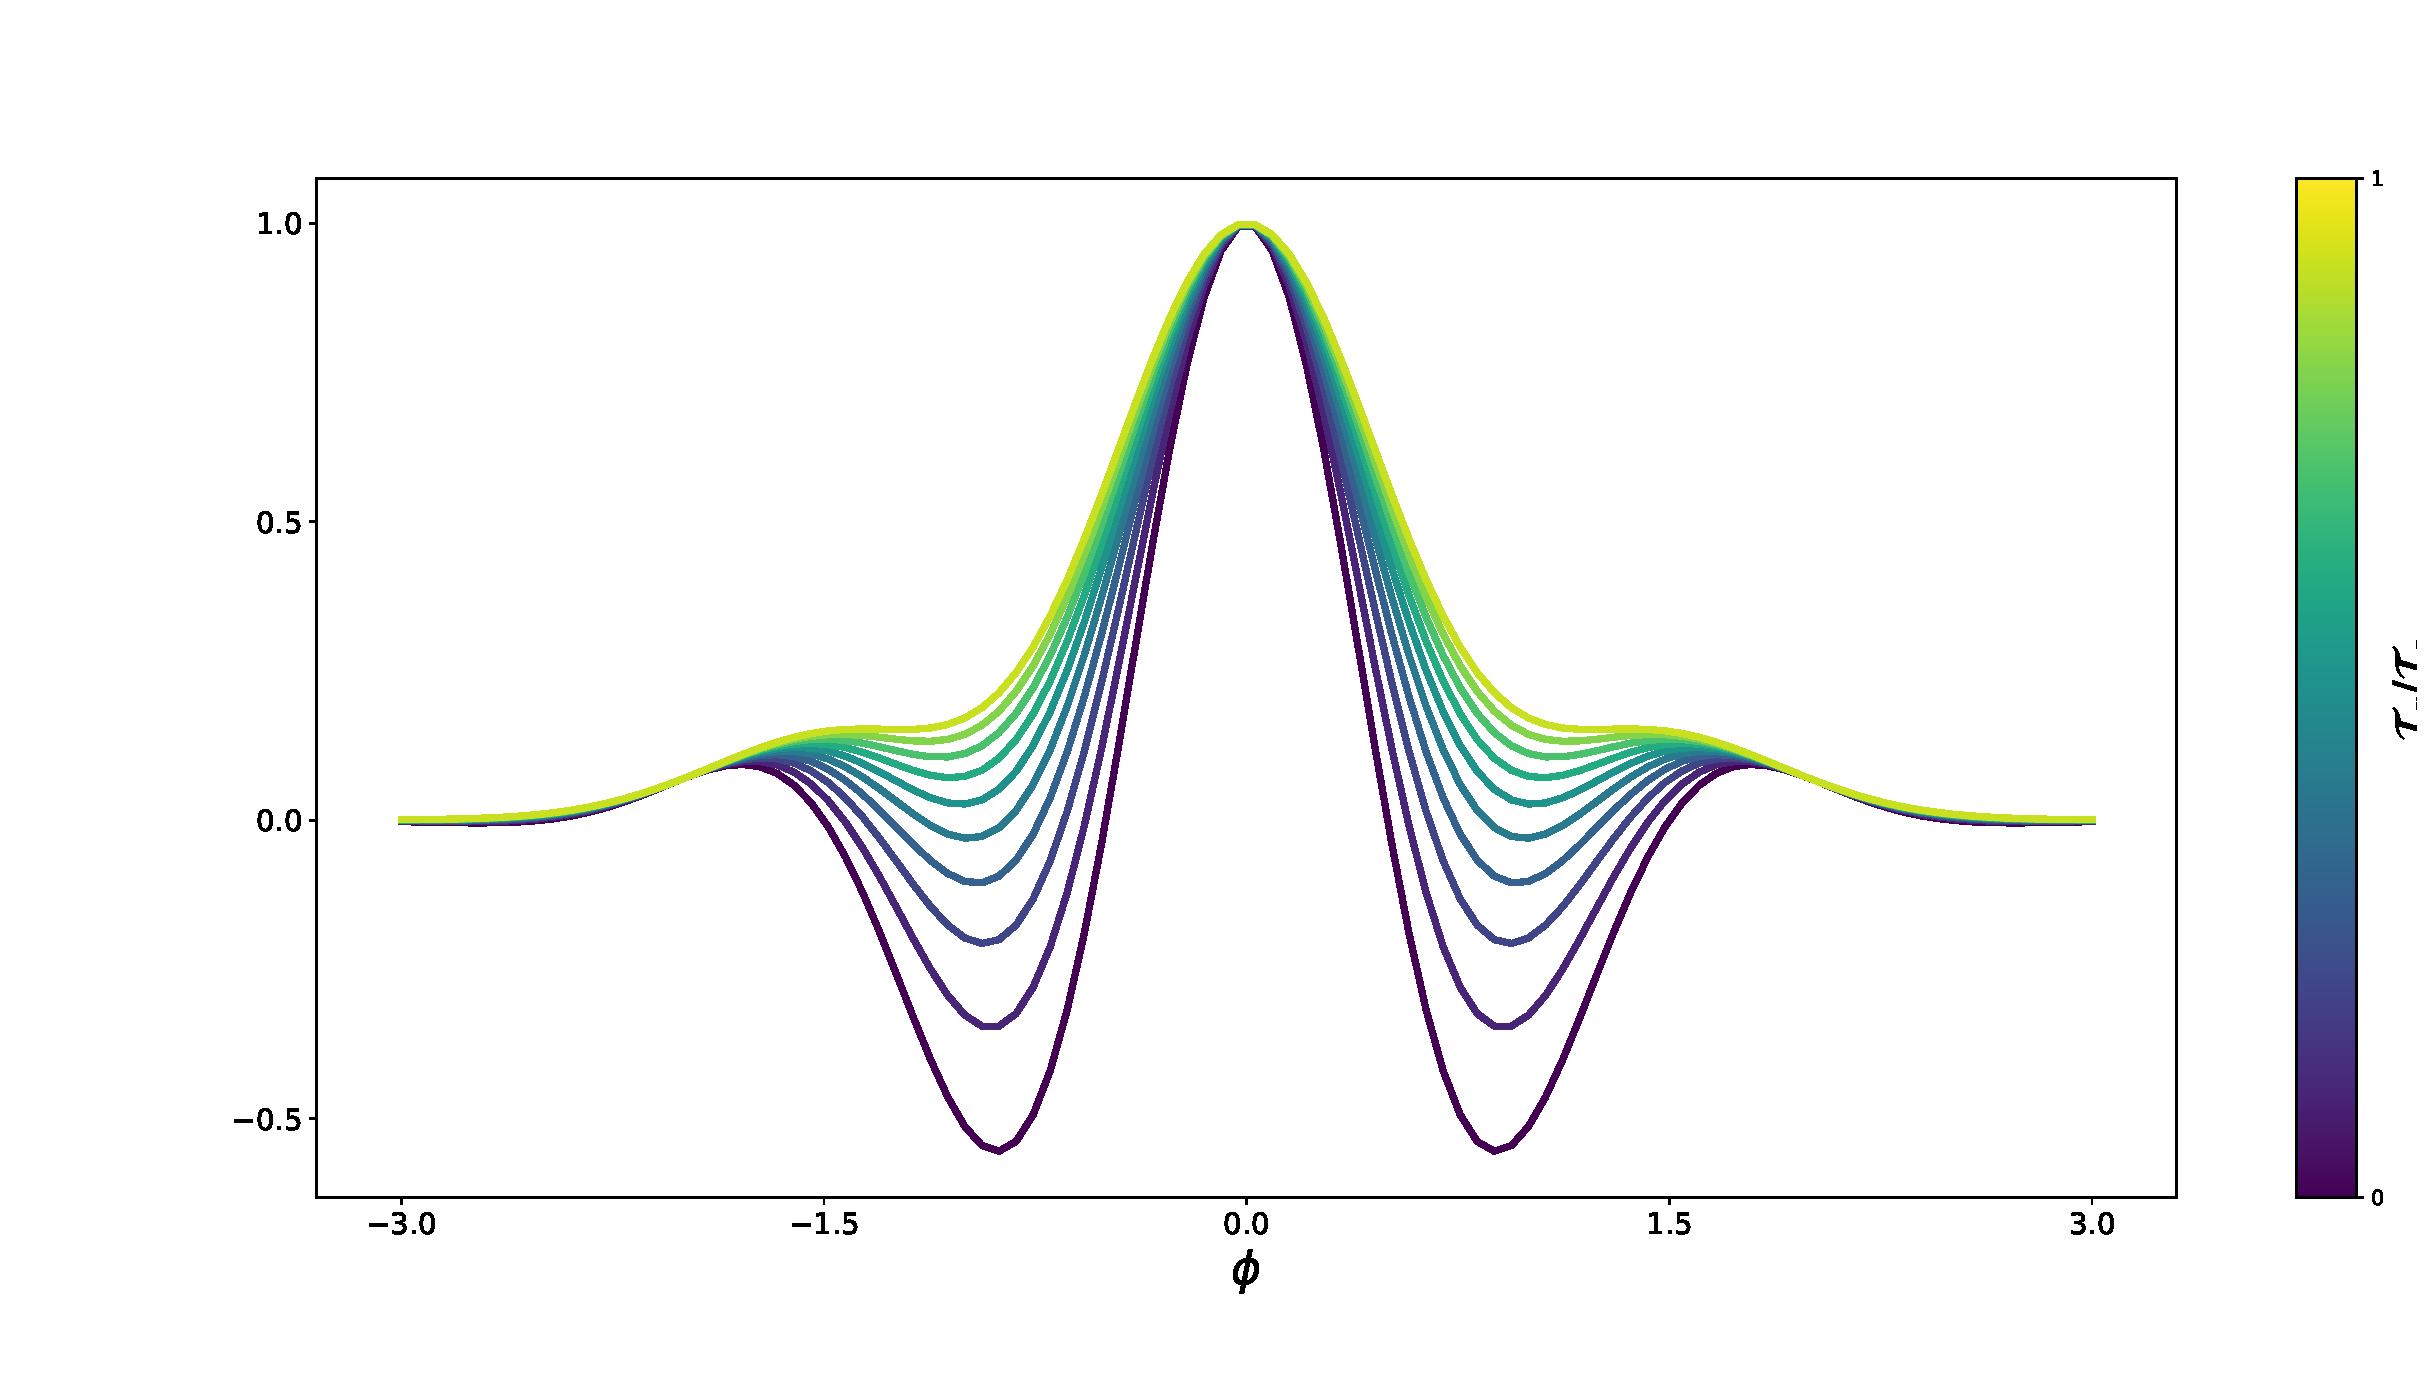
\includegraphics[width=0.8\textwidth]{figure/analyticalmodel/ratio-transmissions-gaussian}
\end{figure}


